\chapter{Implications of codon–anticodon interaction on the regulation of
translation}
\chaptermark{Codon–anticodon interaction}

In the previous chapter I have shown that codon usage and its interaction with
\trna anticodons remains remarkably stable despite substantial variability of
the transcriptome during mammalian development.

Shortly after the publication of our research on \trna gene regulation during
mouse development, \citet{Gingold:2014} published \texttitle{A Dual Program for
Translation Regulation in Cellular Proliferation and Differentiation}. They
report that cells with different functional characteristics preferentially use
different sets of codons, and that the pool of active \trna[s] adapts
dynamically to decode this set of codons with high efficiency.

Because its conclusions are highly relevant to our own research we evaluated the
paper carefully. In the following, I will first describe the paper’s main
findings, to the extent that they are relevant to our own research. I will then
discuss new experimental data and computational analyses we performed to explore
how our previous results relate to this paper.

\section{“A dual program for translation regulation in cellular proliferation
and differentiation”}

\citet{Gingold:2014} investigated the abundance of \trna anticodons and the
codon usage of different groups of protein-coding genes in patient tissue
samples and human-derived cell lines in different cellular conditions --- five
primary cancers, induced differentiation, release from serum starvation,
senescence, and \gene{hsa}{MYC} and \gene{hsa}{RAS} overexpression --- with the
aim of characterising the differences in \trna gene expression and \trna
anticodon abundance. They hypothesise that the balance between \trna anticodon
supply and codon demand might influence the rate of production of proteins from
\mrna \citep{Gingold:2011}.

\subsection{\abbr{trna} anticodons change in abundance in tumour tissues}

\citet{Gingold:2014} designed custom microarrays to probe the expression levels
of the \trna[s] of most anticodons present in human, excluding those prone to
cross-hybridi\-sation, or where a low in silico screening score predicts that
they may be pseudogenes. Using these microarrays, they assayed the abundance of
anticodon isoacceptors in healthy B cells and in B-cell derived lymphomas. They
showed that there are specific anticodon isoacceptors whose abundance changes
reproducibly in tumours compared to healthy tissue, while other anticodon
isoacceptors do not change their abundance. This mirrors results reported
previously \citep{Pavon-Eternod:2009}.

In addition, they determined \trna anticodon abundance analysis levels for all
samples and applied hierarchical clustering to the resulting matrix of \trna
expression profiles. They observed that samples were clustered into two groups,
corresponding to tumour cell types and differentiating cell types. When
performing an equivalent clustering on \mrna gene expression values for the same
samples, they observe that samples cluster not by whether they are tumours, but
rather by their tissue of origin, i.e.\ by the tissue from which the tumour or
cell line was derived.

\subsection{Codon usage differs between genes involved in cell proliferation and
genes involved in differentiation}

Next, \citet{Gingold:2014} looked at protein coding genes within \go terms that
they functionally associated with healthy, adult tissue (“pattern specification
process”) on the one hand, and tumour tissue (“M phase of mitotic cell cycle”)
on the other hand. They show that the codon usage bias in these two \go terms
(averaged over all containing genes) clearly differs
(\cref{fig:go-term-codon-usage}): the genes in both \go terms preferentially use
different synonymous codons.\todo{GO annotation for cell cycle etc will contain + and - regulators}

\textfig{go-term-codon-usage}{body}{0.6\textwidth}
    {Codon usage bias in two \abbr{go} terms.}
    {Each point represents one codon, whose corresponding amino acid is given by
    the label. The position of the point is given by the codon usage bias in
    each \go term, respectively. Codons for the same amino acid share the same
    colour (reproduction of figure 2A in \citet{Gingold:2014}).}

They expand their analysis by calculating the mean codon usage across many \go
categories and perform \pca on the resulting matrix (\cref{fig:go-cub-pca}).
This reveals that the largest contributor to the variation stems from the split
of the \go terms into two distinct sets, one encompassing multi-cellular \go
terms and the other cell autonomous \go terms. They argue that these two sets of
\go terms correspond to \go terms functionally responsible for maintaining cell
homoeostasis on the one hand, and rapid cellular division, such as that found in
tumours, on the other hand. In other words, different gene families specific to
rapidly dividing as opposed to healthy, mature cells have a distinct codon
composition.\todo{GO hierarchy? Term selection? Slice through GO tree --- remove
gene redundancy in sets. Not independent data points [John: “would be very helpful”]}

It is however worth noting that the choice of \go terms highlighted in the \pca
is somewhat arbitrary: It is for instance not clear why “translation” should be
more active during cellular division than in stable cells. The authors rather
describe the relevant set as “cell autonomous” \go terms, but the paper’s
argument implicitly assumes that this corresponds to cell division. Furthermore,
the allocation of genes to \go terms was performed via simple textual matching,
such that \go sub-categories whose description contains the text
“differentiation and proliferation” would be counted as belonging to the \go
super-category “differentiation”.

\textfloat{go-cub-pca}{spill}
    {%
        \begin{minipage}{0.6\textwidth}
            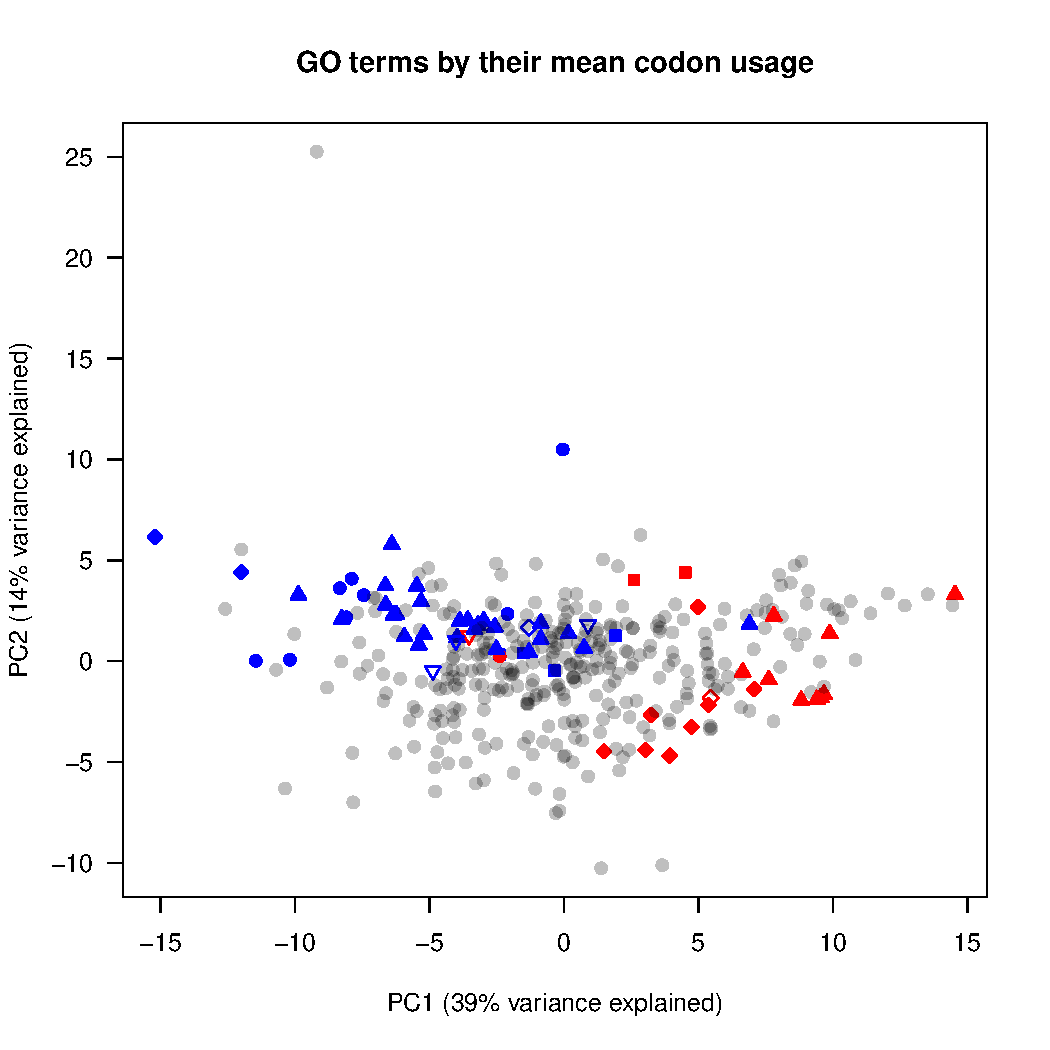
\includegraphics[width=\textwidth]{go-cub-pca}
        \end{minipage}%
        \begin{minipage}{0.4\textwidth}
            \footnotesize\sffamily
            \begin{tabu} to \textwidth {@{}>{\color{blue}\(}c<{\)}X@{}}
                \toprule
                \multicolumn{2}{@{}l}{Multi-cellular} \\
                \quad ▲ & Development \\
                \quad ⬤ & Differentiation \\
                \quad ⬛ & Cell adhesion \\
                \quad ◆ & Pattern specification \\
                \quad ◇ & Multicellular organism growth \\
                \quad ▽ & Angiogenesis \\
                \addlinespace
            \end{tabu}
            \begin{tabu} to \textwidth {@{}>{\color{red}\(}c<{\)}X@{}}
                \multicolumn{2}{@{}l}{Cell autonomous} \\
                \quad ▲ & Mitotic cell cycle \\
                \quad ⬤ & Nucleosome assembly \\
                \quad ⬛ & Chromatin remodelling/modification \\
                \quad ◆ & Translation \\
                \quad ◇ & \mrna metabolic process \\
                \quad ▽ & Negative regulation of cell cycle \\
                \bottomrule
            \end{tabu}
        \end{minipage}
    }
    {\pca of mean \go term codon usage.}
    {Each dot corresponds to one \go term. The position of the dots is derived
    by rotating the matrix of the mean codon usage of the genes belonging to
    each \go term. Created using methods of \citet{Gingold:2014} (the precise
    numbers differ slightly due to the use of different implementations to
    perform the analysis but this does not impact the interpretation).}

\subsection{Differential codon usage in cell-condition specific gene sets
matches \abbr{trna} anticodon abundance in corresponding cells}

Finally, \citet{Gingold:2014} compared the \pca of the per-\go codon usage to
the actual gene expression of \mrna[s] and \trna[s] in different cellular
conditions. The analysis was done in two parts. Firstly, the fold change of gene
expression between normal tissue and a given condition was calculated for each
protein-coding gene. The mean expression fold change of each \go term, mapped to
a colour map, was plotted on top of the \go terms in the \pca
(\cref{fig:gingold-3c} bottom). This was done separately for various
conditions, including several tumour samples and cell lines with induced
differentiation. In all examined conditions, there seems to be a marked gradient
of \mrna expression enrichment from left to right. This illustrates that the
first principal component of the \pca does indeed separate \go terms by their
specificity to either proliferating or differentiating cellular
programmes.\todo{John: Does it? Assuming “normal” cells are proliferating? Does
this not beg the question of comparing tumour/differentiating directly?}

Secondly, to estimate translation efficiency they calculated the change in
abundance of the \trna genes whose isoacceptors decode the codons of the genes
in each \go term, and averaged across them.\todo{Unclear, add equations} The fold change in translation
efficiency between healthy tissue and the sample under consideration was again
mapped to a colour gradient, which was overlaid over the \pca
(\cref{fig:gingold-3c} top). Again there appears to be a gradient of how
well different \go terms are adapted to the \trna anticodon pool of a given
condition, following the first principal component of the \pca.

Although interesting, the authors did not calculate correlations between the
first principal component and either the codon usage bias or the translation
efficiency fold change. Instead, they visualised the presumed correspondence
using a potentially misleading rainbow colour map \citep{Borland:2007}.
Furthermore, the absolute range of changes is extremely small compared to the
overall fold change (range of fold change \numrange{0.86}{0.905} in one case,
corresponding to less than \num{5} per cent of the maximum fold change), and the
lack of statistical analysis makes it impossible to tell whether these changes
are in fact significant. It is also important to note that the fold change range
in predicted translation efficiency is positive: Consequently, \go categories
that are unspecific for a given condition according to \cref{fig:go-cub-pca},
and should thus be less adapted to the \trna anticodon abundance, are in fact
better adapted according to this analysis (\cref{fig:gingold-3c}). This is a
recurring feature for all conditions tested in this way, and is potentially
inconsistent with the claim that the \trna anticodon pool is specially adapted
to cell condition specific gene sets.

\textfloat{gingold-3c}{body}{%
    \centering
    \begingroup
        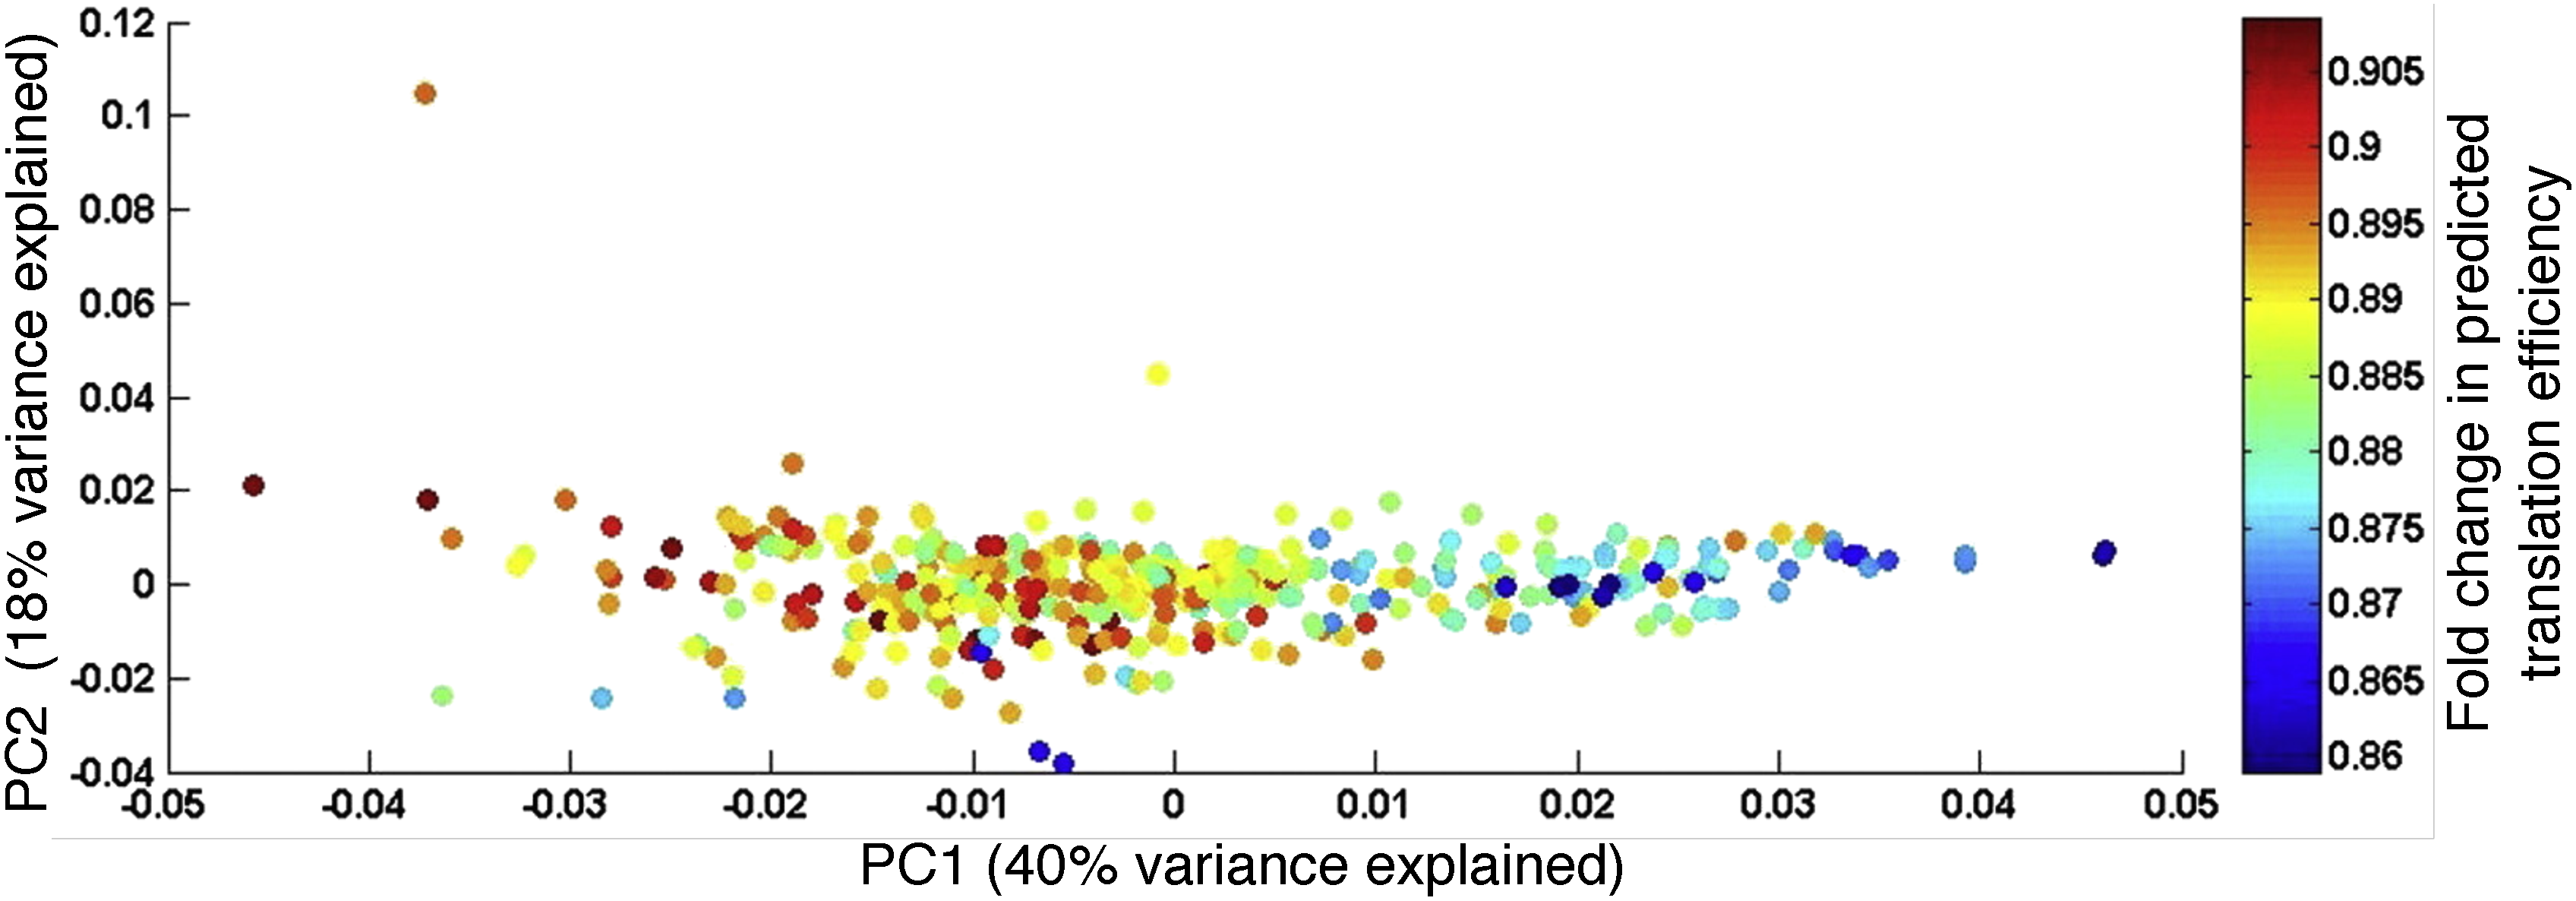
\includegraphics[width=\textwidth]{gingold-3c-trna}\\[-0.3\baselineskip]
        \subcaption{\label{fig:gingold-3c-a}Fold change in predicted translation
            efficiency}\leavevmode\\
    \endgroup
    \begingroup
        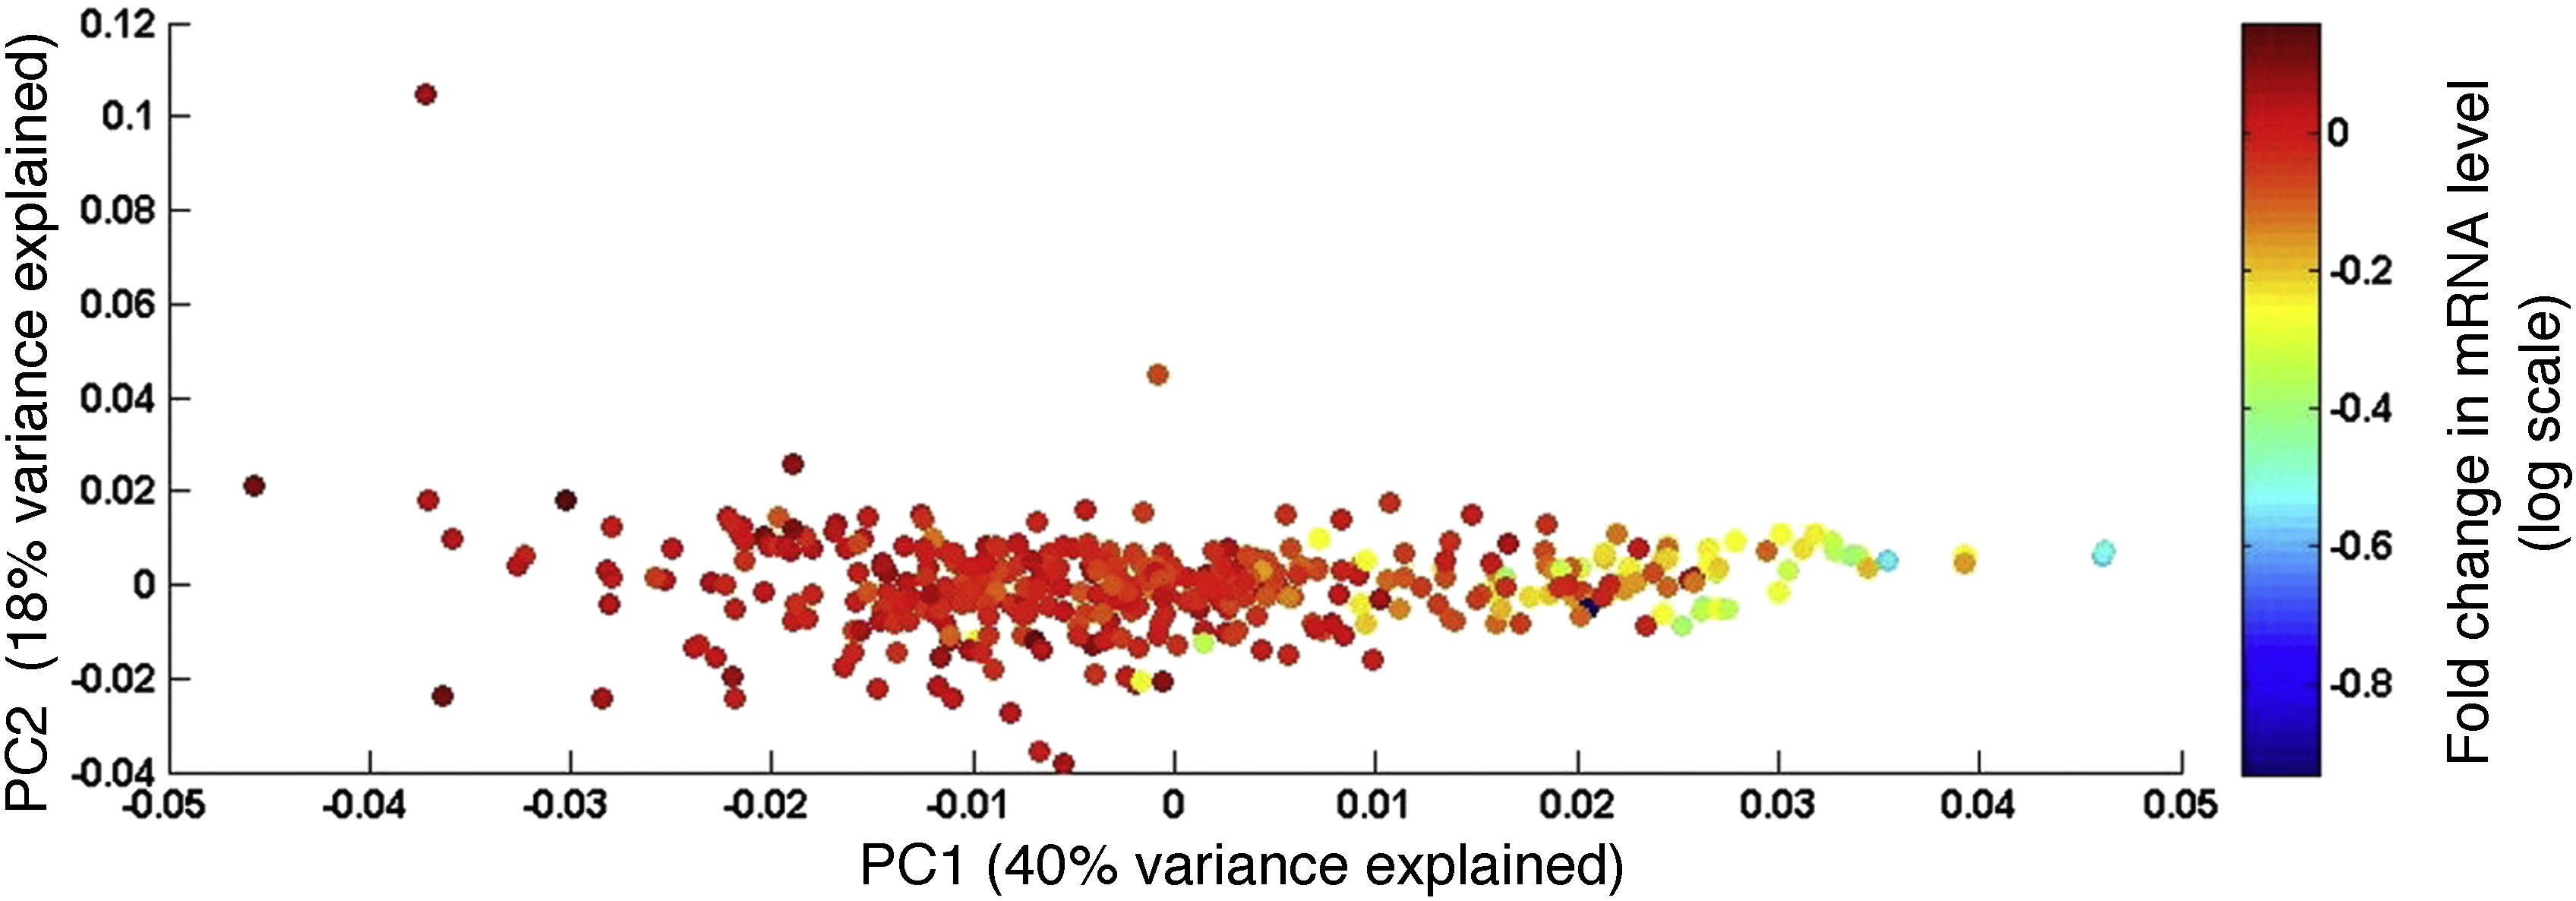
\includegraphics[width=\textwidth]{gingold-3c-mrna}\\[-0.3\baselineskip]
        \subcaption{\label{fig:gingold-3c-b}Fold change in \abbr{mrna} level}
    \endgroup}
    {Projection of the \trna and \mrna expression changes on the codon usage
    map for cells after induced differentiation via retinoic acid.}
    {Both panels show the same \pca that I reproduced in \cref{fig:go-cub-pca}.
    In the top panel, the colours correspond to the fold change in predicted
    translation efficiency of the genes constituting each \go term, given the
    change in cellular abundance of \trna anticodons compared to normal cells.
    The bottom panel shows the mean fold change in \mrna levels per \go term
    compared to normal cells. Figure modified from \citet{Gingold:2014}.}

\section{Are \abbr{trna} anticodon abundance and codon usage highly adapted to
different cellular conditions?}

To explore how these two findings — the stability of the anticodon pool through
development on the one hand \citep{Schmitt:2014}, and the malleability of the
anticodon pool to match the codon demand of highly expressed protein-coding
genes on the other hand \citep{Gingold:2014} — we examined differences between
healthy tissue and tumour cell lines in \mmu and \hsa.

\subsection{The effect of gene set size on codon usage bias}

Since we were already in possession of relevant \trna data we decided to use our
own data to recapitulate these findings. A first observation was that we had
looked at the whole transcriptome, \citet{Gingold:2014} had looked at specific
subsets. While both approaches are valid, some caution is necessary when
comparing the results: the smaller the set of genes, the larger the effects of
random sampling of the genes become. Subsequently, when analysing a particular
feature, such as codon usage bias, random sampling will contribute
proportionally more to the variation between two small sets than to differences
between two larger sets. Consequently, if one wants to assert that deviations
are nonrandom, one thus has to account for this effect.

To assess how much of the variation in \go term codon usage is explainable by
such effects, I generated random sets of different numbers of genes,
corresponding to the whole range of \go term gene set sizes. For each simulated
gene set, I calculated the total codon usage of the genes in the resulting set.
To ensure that the codon usage of different gene sets was comparable, all codon
frequencies within a sample were normalised by the total codon frequency in the
sample, to obtain codon proportions:

\begin{equation}
    x_i^* = \sum_{g\in G} x_{ig} \left(\sum_j \sum_{g\in G} x_{jg}\right)^{-1}
\end{equation}

Where \(i, j \in \codon{AAA},\dots,\codon{TTT}\) are the codons (excluding stop
codons), \(g\in G\) are the genes in the sample, \(x_{ig}\) is the codon
frequency of codon \(i\) in gene \(g\), and \(x_i^*\) is the relative codon
frequency of codon \(i\) in the sample. We have \(\sum_i x_i^*=1\).

This was done \num{10000} times for each \go term gene set size. Next, I
calculated the Pearson correlation between the codon proportions of each sample
with the genome-wide codon proportions (across all annotated coding sequences).
\Cref{fig:sample-size-dependent-cub} plots the distribution of the correlations
against the gene set sizes.

\textfig{sample-size-dependent-cub}{spill}{\textwidth}
    {Dependence of codon usage variability on sample size.}
    {Genes were randomly sample from the human genome to create sets of sizes
    given by \(x\) (in grey). The mean codon usage of the sets was calculated,
    and their Pearson correlation to the genomic background is shown on the
    \(y\) axis. For each size, the distribution of \num{10000} repeated samples
    is summarised in the figure by a vertical segment connecting the first with
    the third quartile; the mean is indicated as a black dot. The second and
    ninety eighth percentile are hinted at with smaller dots.}

I used these distributions to calculate empirical \(p\)-values for each \go term
in order to test the null hypothesis \(H_0\): the divergence in codon usage from
a background distribution is indistinguishable from random variation for this
\go term. \Cref{fig:significant-go-term-cub-var} plots the codon usage variation
of each \go term, along with an indication of whether the observed variation is
explained by random variation alone.

\textfig{significant-go-term-cub-var}{spill}{\textwidth}
    {\go term codon usage variation.}
    {Each point corresponds to a \go term whose Pearson correlation of codon
    usage with the genomic background is plotted against its gene set size.
    \go terms with an \fdr-adjusted \(p < 0.05\) are coloured in red.}

The plot illustrates that the variation of many \go terms is expected by chance;
however, more than half (\num{421} out of \num{791}, \num{53} per cent) show
significantly higher variation. Thus, despite an influence of random sampling
especially for small gene set sizes, this observation is unlikely to explain the
variation seen in \cref{fig:go-cub-pca}.

\subsection{The extent of anticodon adaptation to distinct cellular conditions}

Next, in order to test whether the anticodon pool adapts to specific cellular
conditions as suggested by \cref{fig:gingold-3c}, I examined whether the
codon--anticodon adaptation is better between matching than between mismatching
\mrna and \trna transcriptomes. For this purpose, I calculated codon--anticodon
adaptation as the correlation between matching codons and anticodons, each as a
proportion of the contribution to their corresponding amino acid -- in other
words, the correlation between \rcu and \raa. I similarly tested whether the
codon--anticodon adaptation was better for genes that are specific to a cellular
condition, compared to the overall transcriptome. In other words, I looked at
the \mrna pool of each cellular condition, and calculated the codon--anticodon
correlations for

\begin{enumerate}
    \item the whole transcriptome and its matching \trna pool (“matching”),
    \item the whole transcriptome and all mismatching \trna pools
        (“mismatching”),
    \item the set of differentially, highly expressed \mrna genes and the
        \trna pool of the same cellular condition (“\abbr{de}”), and
    \item a condition specific gene set (for the \go terms “M phase of mitotic
        cell cycle” \& “pattern specification process”) and the \trna pool of
        the same cellular condition (“\abbr{go}”).
\end{enumerate}

I performed the analysis using data generated from \mmu and \hsa. For both
species, I compared healthy tissue (adult whole-liver tissue, homogenised) to
two different hepatocyte derived cancer cell lines: HepG2 and Huh7 in \hsa, and
Hepa1-6 and Hepa1c1c7 in \mmu. At least two biological replicates were present
for each sample.\footnote{The tissue collection and sequence library preparation
was performed by Bianca Schmitt and Diego Villar.}\todo{John: More details} Distinct tumours were used
because we wanted to test the hypothesis that there exists a \trna abundance
adaptation specific to the cellular programme in proliferating cells, which
would be present across different tumour types.

The analysis compares different scenarios that should, according to the
hypothesis proposed by \citet{Gingold:2014}, show markedly different
distributions: codon and anticodon pools of the same cellular conditions should
be highly coordinated (correlation type “matching”). Codons and anticodons of
\emph{mismatching} conditions (i.e.\ the codon pool of a healthy cell and the
anticodon pool of a tumour cell, or vice versa) should be less well coordinated
(correlation type “mismatching”). Furthermore, the codon usage of just a subset
of the overall transcriptome corresponding to genes specific to the cellular
condition should be coordinated with their anticodon pool to an even greater
extent. Conversely, if we did not expect a \trna anticodon pool adapted to
specific subsets of the transcriptome, we might expect that the correlation
between the codon usage of such subsets and the anticodon abundance was
\emph{less} than that of the overall transcriptome, due to higher stochastic
variability in smaller gene sets.

Cell specific subsets of the transcriptome can be defined in several ways. My
analysis used two possible definitions: Firstly, I looked at differentially
expressed genes between healthy and tumour cells, and called genes
condition-specific if they were significantly differentially expressed (adjusted
\(p < 0.001\)), their expression was high (mean expression across conditions in
the upper quartile of all mean expression levels), and their fold change between
the conditions was also high (taking the \num{200} genes with the highest fold
change; correlation type “\abbr{de}”). Secondly, I took the gene sets of the two
most extreme \go terms found by \citet{Gingold:2014} according to the variance
in codon usage, which they describe as highly specific for proliferating cells
(\go term “M phase of mitotic cell cycle”) and differentiating/differentiated
cells (\go term “pattern specification process”; correlation type “\abbr{go}”).

Unfortunately, \go term annotations differ vastly between \hsa and \mmu and, in
particular, one of the two condition specific \go terms (according to the \pca
analysis, \cref{fig:go-cub-pca}) is badly annotated in \mmu (with only \num{3}
genes annotated for “M phase of mitotic cell cycle”). As a consequence, I did
not use the existing \go term annotations for mouse but rather used the
orthologous gene sets from the human \go term annotation (determined from the
gene name, which is identical in \mmu and \hsa \citep{Wain:2002}).

We want to test whether the “mismatching” correlations are lower than the
“matching” ones and whether the “\abbr{de}” and “\abbr{go}” correlations are
higher, respectively, than the “matching” ones. I therefore used one-tailed
tests for significant deviations from the null. In all but one cases, I failed
to reject the null hypothesis of no difference. The only case where we find some
support for rejecting \(H_0\) is the comparison of “matching”--“mismatching” in
\hsa (\(p = 0.048\), one-tailed Mann–Whitney–Wilcoxon test). On the other hand,
the “\abbr{go}” correlations are significantly \emph{lower} than the “matching”
correlations in both species (\(p < \num{4.4e-5}\) in \mmu; \(p < \num{2.5e-8}\)
in \hsa). This offers evidence against the hypothesis put forward by
\citet{Gingold:2014} (\cref{fig:cub-aab}).

\textfloat{cub-aab}{spill}
    {%
        \begin{minipage}{0.35\textwidth}
            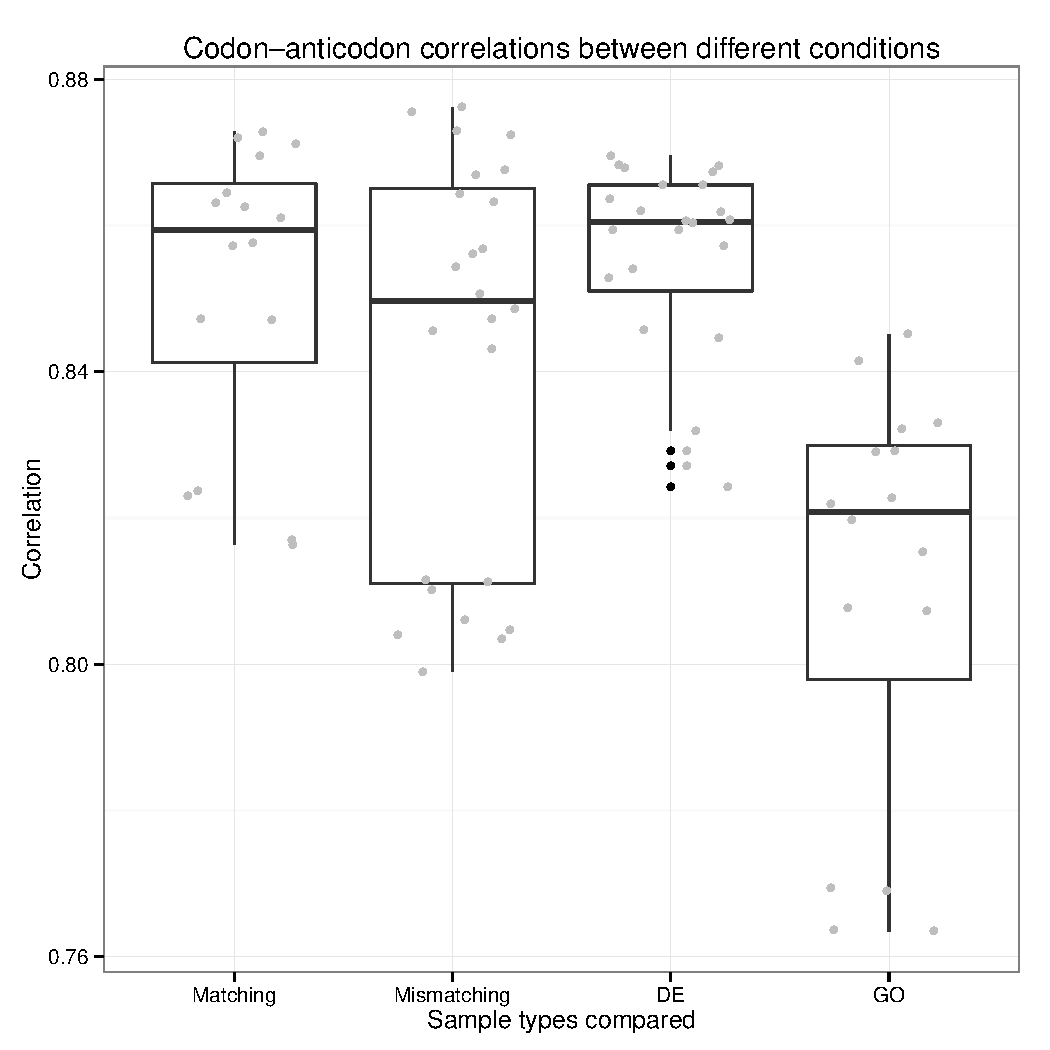
\includegraphics[width=\textwidth]{cub-aab-mouse}%
            \subcaption{\mmu}
        \end{minipage}%
        \begin{minipage}{0.35\textwidth}
            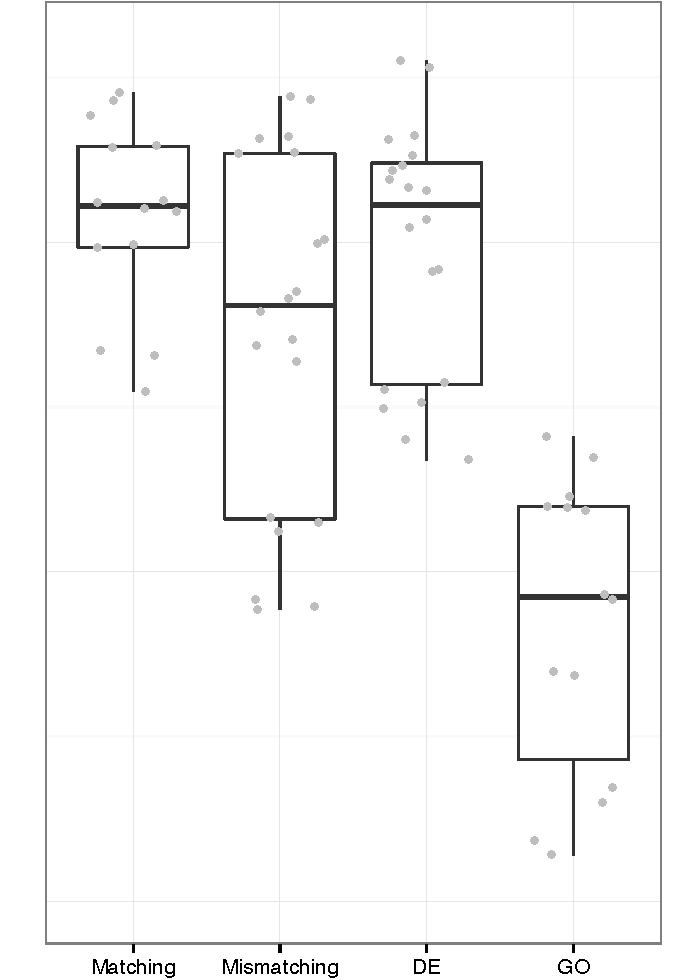
\includegraphics[width=\textwidth]{cub-aab-human}%
            \subcaption{\hsa}
        \end{minipage}%
        \begin{minipage}{0.3\textwidth}
            \scriptsize\sffamily
            \begin{tabu} to \textwidth {@{}ll@{\ --\ }l@{}}
                \toprule
                    %& \multicolumn{2}{c}{Contrast} \\
                    & \multicolumn{1}{l@{}}{\abbr{mrna}} & \abbr{trna} \\
                \midrule
                Matching \\
                \quad\mmu & healthy liver & healthy liver \\
                     & Hepa1-6 & Hepa1-6 \\
                     & Hepa1c1c7 & Hepa1c1c7 \\
                \quad\hsa & healthy liver & healthy liver \\
                     & HepG2 & HepG2 \\
                     & Huh7 & Huh7 \\
                \addlinespace
                Mismatching \\
                \quad\mmu & healthy liver & Hepa1-6 \\
                     & healthy liver & Hepa1c1c7 \\
                \quad\hsa & healthy liver & HepG2 \\
                     & healthy liver & Huh7 \\
                \bottomrule
            \end{tabu}
        \end{minipage}
    }
    {Codon--anticodon correlations.}
    {Each box shows a distribution of codon--anticodon Spearman correlations.
    A codon--anticodon correlation is computed from relative contributions to
    the respective amino acid (i.e.\ \abbr{rcu} versus \abbr{raa}), ignoring
    wobble base pairing. “Matching” shows correlations of the codon and
    anticodon pool of the same condition. “Mismatching” shows correlations of
    the codon and anticodon pool of mismatching conditions (e.g. Hepa1-6 codons
    versus healthy liver anticodons); the two cancer replicates are \emph{not}
    counted as mismatching conditions. “\abbr{de}” shows correlations of the
    codon pool of highly, differentially expressed \mrna genes, and the
    anticodon pool of the same condition. “\abbr{go}” shows correlations of the
    codon pool of condition-specific \abbr{go} term gene sets, and the anticodon
    pool of the same condition. For all distributions, correlations were
    calculated between all pairwise combinations of replicates.}

It is worth nothing that the “\abbr{de}” codon--anticodon correlations vary
non-negligibly, depending on how exactly the top \num{200} condition-specific
genes are chosen; alternative strategies to the one outlined were not found to
change the overall result, however: none of the strategies yielded correlations
that were significantly higher than the transcriptome-wide “matching”
correlations.

\subsection{Other genomic features may drive the perceived codon usage bias}

The trend seen in \cref{fig:go-cub-pca} exists, albeit to a lesser degree, when
plotting amino acid usage rather than codon usage (\cref{fig:go-aa-pca}). The
first principal component separates the \go term “keratinisation” from the rest.
This is due to the fact that the proteins in this \go term are uniquely highly
enriched in the amino acid proline, which forms more rigid peptide bonds than
all other amino acids, with implications for the robustness of, amongst other
things, the cellular skeleton. The proteins in this \go term are thus implicated
in the structural formation of the epithelium \citep{Hohl:1995}. The second
principal component, by contrast, shows the same separation of \go categories as
the first principal component of \cref{fig:go-cub-pca}. Moreover, these two
principal components are highly correlated (Pearson’s \(\rho = 0.95\)). Clearly,
this correlation cannot be explained by \emph{codon} identity, since amino
acids, not codons, conventionally determine protein function. However, amino
acid usage alone does not explain the pattern either: After removing amino acid
identity as a confounding factor (by computing \rcu instead of codon usage), the
\go term \pca still displays the previously observed separation of \go
categories (\cref{fig:go-rcu-pca}).

\textfigtwo{go-aa-pca}
    {\pca of mean \go term amino acid usage.}
    {Each dot corresponds to one \go term. The position of the dots is derived
    by rotating the matrix of the mean amino acid usage of the genes belonging
    to each \go term. Colours and symbols as in \cref{fig:go-cub-pca}.}
    {go-rcu-pca}
    {\pca of mean \go term \rcu.}
    {Each dot corresponds to one \go term. The position of the dots is derived
    by rotating the matrix of the mean \rcu of the genes belonging to each \go
    term. Colours and symbols as in \cref{fig:go-cub-pca}.}

We thus conclude that both changes in codon usage and changes in amino acid
usage independently correlate with the separation of \go terms into two
functional categories. Furthermore, given the results presented in the previous
chapter, we note that we have no evidence for a functional adaptation of the
\trna pool to specific gene sets. I therefore looked for other factors that
could explain the observed patterns in codon usage. It has previously been
reported that gene codon usage can be predicted by the intergenic sequence \gc
bias in prokaryotes \citep{Chen:2004}. They remark that the finding cannot be
directly translated into mammals due to the variability in \gc bias between
distinct, large regions across the genome. However, despite these large-scale
variations of the \gc bias, local regions exhibit a stable \gc bias in mammalian
genomes. Consequently, \gc bias could still play a role in codon deployment.

In fact, the first principal component of the codon usage spread
(\cref{fig:go-cub-pca}) as well as the second principal component of amino acid
spread (\cref{fig:go-aa-pca}) correlate highly with the \gc bias in the \go term
gene sets (Pearson’s \(\rho = -0.96\), \(\rho = -0.58\);
\cref{fig:cu-vs-gc,fig:aa-vs-gc}). This suggests that genomic features other
than gene function might influence gene codon usage. However, it is entirely
conceivable that the differences in \gc bias of the \go terms are caused by the
changes in either amino acid or codon usage, rather than the other way round:
any genetic point mutation from \nA or \nT to \nC or \nG (or vice versa) by
definition changes the \gc content of that region. We thus do not expect
changing codon composition to be \gc neutral.

To establish whether the driver of this correlation is large-scale \gc bias
adaptation, changes in protein function and thus amino acid usage or subtle
changes in codon usage to regulate translation, we therefore need to examine the
\gc bias of the intergenic regions surrounding each \go term’s genes: not being
part of any \mrna transcript, the \gc bias of the intergenic regions cannot be
driven by codon-level selection. It can thus serve as a background for the
expected variation in \gc to compare against the \gc variation that we see
between \go terms. An outline of the necessary investigation to answer this
question can be found in the conclusion in \cref{sec:conclusion}.

\textfloat{cub-vs-gc}{spill}
    {%
        \begin{minipage}{0.5\textwidth}
            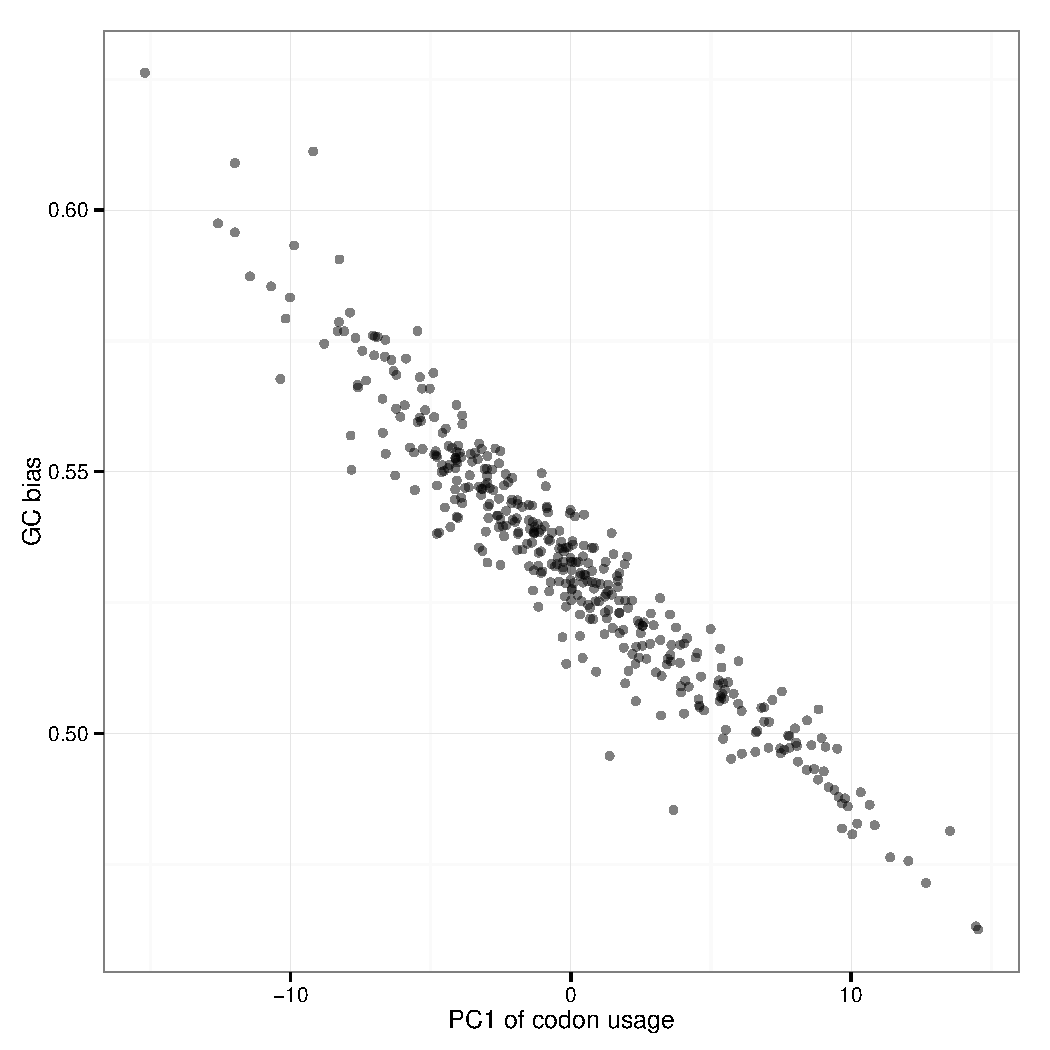
\includegraphics[width=\textwidth]{cub-pc1-vs-gc}%
            \subcaption{\label{fig:cu-vs-gc}\gc bias against codon usage
            (Pearson’s \(\rho = -0.96\)).}
        \end{minipage}%
        \begin{minipage}{0.5\textwidth}
            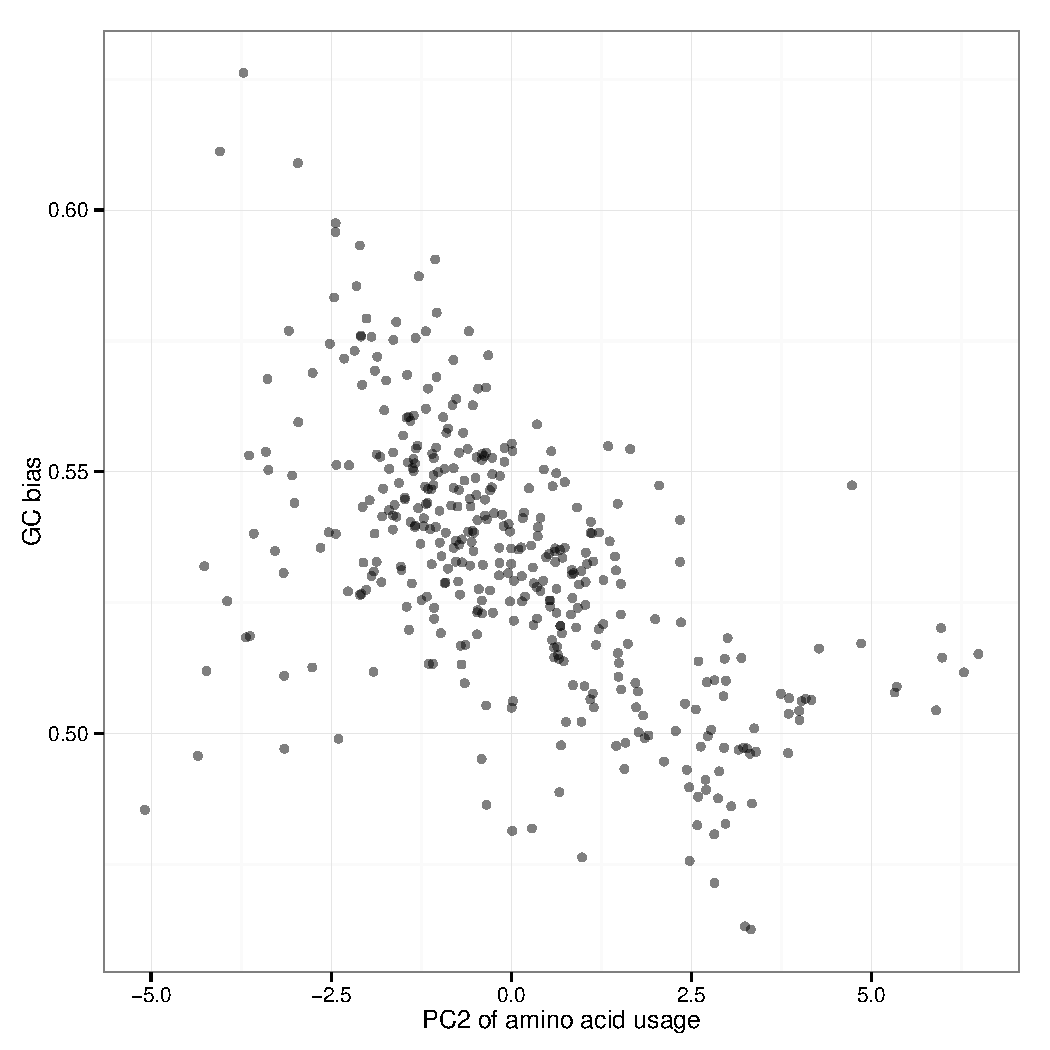
\includegraphics[width=\textwidth]{aa-pc2-vs-gc}%
            \subcaption{\label{fig:aa-vs-gc}\gc bias against amino acid usage
            (Pearson’s \(\rho = -0.58\)).}
        \end{minipage}%
    }
    {\gc bias against a principal component of the \go term codon \& amino acid
    usage \pca.}
    {Each point represents one \go term. The \(x\) coordinate corresponds to
    that of the named principal component of the \pca in
    \cref{fig:go-cub-pca,fig:go-aa-pca}. The \(y\) coordinate corresponds to
    the mean \gc bias of the \go gene set.}

\subsection{Discussion}

In this chapter I extended the analysis from \cref{sec:trna}, and contrasted it
with the findings by \citet{Gingold:2014}. We have moved beyond the variation of
\trna gene expression and have questioned the apparent stability of the codon
usage and anticodon isoacceptor abundance in the transcriptome in the face of
major changes in cell function. However, contrary to previous reports I was
unable to find evidence for a selective adaptation of the \trna pool to
cell-specific subsets of genes. The work presented in this chapter constitutes
just the start of our investigation into the codon usage variability of subsets
of the transcriptome. Many questions still remain open.

\subsubsection{Codon--anticodon adaptation to distinct cellular conditions}

One caveat of the analysis of the codon--anticodon correlation between subset of
the transcriptome is the treatment of replicates. In \cref{fig:cub-aab},
biological replicates of each sample were treated independently, rather than
pooled: correlations were calculated between all pairwise combinations of
\rnaseq and \pol3 \chipseq data of the samples under consideration. Each data
point thus corresponds to a pairwise combination of two replicates; this implies
that data points within one distribution are \emph{not} independent of each
other. The alternative would have been to average over biological replicates,
and correlate the averaged data. However, this has two important drawbacks:

\begin{enumerate}
    \item It does not account for variance in the expression data and thus
        underestimates the variance in the distributions of the correlations.
    \item If \mrna and \trna gene expression values are dispersed around the
        same mean, averaging across replicates would yield a higher correlation
        than actually present in vivo.
\end{enumerate}

The current analysis measured \trna anticodon adaptation using the
codon--anticodon correlation, ignoring wobble base pairing. A potentially better
measure of \trna adaptation is the \tai, which accounts for wobble base pairing
in a species-specific manner. Extending the analysis to use the \tai is ongoing
work.

\subsubsection{Evolutionary conservation of \abbr{trna}--codon adaptation}

If a mechanism leading to the adaptation of the cellular \trna pool to different
cellular conditions existed, we would expect this to be well conserved across
mammalian evolution. Indeed, if the \trna pool is differentially adapted to the
codon usage of subsets of genes, then the codon usage of these genes would be
under negative selection, and should thus show conservation. Furthermore, this
conservation should therefore be \emph{stronger} than genomic features under
neutral selection, such as \gc content. Thus, if we can show that codon usage
bias of \go term gene sets is no more conserved across mammalian evolution than
\gc bias, this may provide additional evidence against the hypothesis of a
functional relevance for gene set specific codon bias.

Using genome data from different mammalian species and homology information for
the annotated \go categories in humans, we are able to infer how strongly
conserved codon usage is compared to the conservation of other genomic features
such as \gc bias for each orthologous gene. Under the assumption that codon
usage is selected for to drive differential translation rates in different
cellular conditions, we would expect a comparatively high correlation of codon
usage compared to other genomic features.
